\section{Derivation of the Compton Formula}
\subsection*{A photon collides with an electron}

\begin{center}
	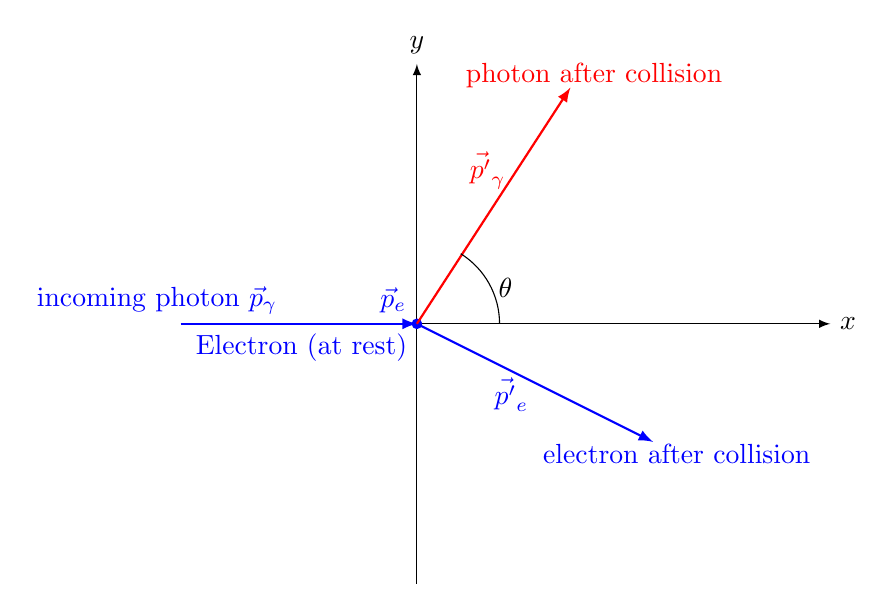
\begin{tikzpicture}[scale=1.5, >=latex]
		% Axes
		\draw[->] (-0.2,0) -- (3.5,0) node[right] {$x$};
		\draw[->] (0,-2.2) -- (0,2.2) node[above] {$y$};
		
		% Origin = electron before collision
		\filldraw[blue] (0,0) circle (0.04) node[below left] {Electron (at rest)};
		
		% Incoming photon
		\draw[->, thick, blue] (-2,0) -- (0,0);
		\node[blue] at (-2.2, 0.2) {incoming photon $\vec{p}_\gamma$};
		
		% Electron after collision
		\draw[->, thick, blue] (0,0) -- (2,-1);
		\node[blue] at (0.8,-0.6) {$\vec{p'}_e$};
		\node[blue] at (2.2,-1.1) {electron after collision};
		
		% Photon after collision
		\draw[->, thick, red] (0,0) -- (1.3,2) ;
		\node[red] at (0.6,1.3){$\vec{p'}_\gamma$};
		\node[red] at (1.5,2.1) {photon after collision};
		
		% Scattering angle theta (between x-axis and scattered photon)
		\draw (0.7,0) arc (0:57.995:0.7);
		\node at (0.75,0.3) {$\theta$};
		\node[blue] at (-0.2,0.2) {$\vec{p}_e$};
	\end{tikzpicture}
\end{center}

\subsection{Energy transfer in the Compton effect}

The incident photon has higher energy (and thus higher frequency) than the scattered photon after the collision. Part of the photon’s energy is transferred to the electron, so the photon loses energy. Since a photon’s energy is proportional to its frequency,
\[
E = h \nu,
\]
the frequency of the scattered photon decreases after the collision—and its wavelength correspondingly increases.
\begin{DidacticBox}[Energy vs.\ frequency]
	A photon loses energy \(\Delta E\) in the collision; since \(E = h\nu\), its frequency drops and the wavelength grows (\(\lambda' > \lambda\)).
	This is the central intuition behind the ensuing shift \(\Delta\lambda\).
\end{DidacticBox}

\subsection{Energy conservation in the collision}
\[
E_\gamma + E_e = E'_\gamma + E'_e
\]

\begin{align*}
	E_\gamma &: \quad \text{energy of the incident photon} \\
	E_e       &: \quad \text{energy of the electron before the collision} \\
	E'_\gamma &: \quad \text{energy of the scattered photon} \\
	E'_e      &: \quad \text{energy of the electron after the collision}
\end{align*}
For notational convenience, define:
\begin{align*}
	p_\gamma &= \lVert \overrightarrow{p}_\gamma\rVert\\
	p_e &= \lVert \overrightarrow{p}_e\rVert
\end{align*}

\subsection{For the massless photon:}
\begin{align*}
	E_\gamma = \sqrt{m^2c^4 + c^2 p_\gamma^2} = c\,p_\gamma \quad \text{since } m=0
\end{align*}

\subsection{For the electron at rest:}
\begin{align*}
	E_e = m_e c^2
\end{align*}

\subsection{For the electron after the collision:}
\begin{align*}
	E'_e = \sqrt{m_e^2 c^4 + c^2 p_e'^2}
\end{align*}

\subsection{Energy conservation becomes}
\begin{align}
	E_\gamma + E_e &= E'_\gamma + E'_e \nonumber\\
	c p_\gamma + m_e c^2 &= c p'_\gamma + \sqrt{m_e^2 c^4 + c^2 {p'_e}^2} \label{Energie}
\end{align}
Goal: relation among $p_\gamma$, $p'_\gamma$, and the angle $\theta$. Thus we must eliminate $p'_e$.\\

\subsection{Momentum conservation}
Choose a convenient coordinate system:
\begin{itemize}
	\item Electron at the origin
	\item Photon travels along the $x$-axis directly toward the electron
\end{itemize}

\begin{center}
	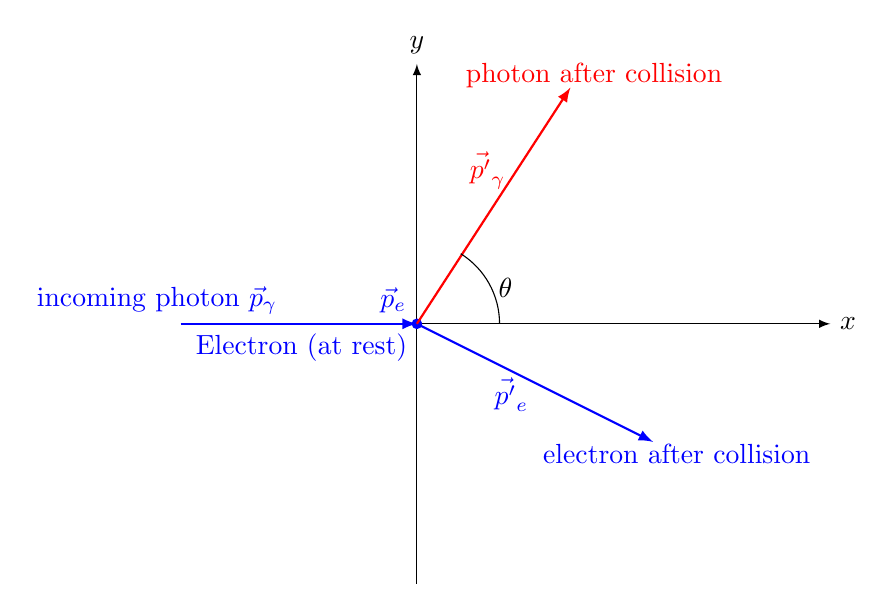
\begin{tikzpicture}[scale=1.5, >=latex]
		% Axes
		\draw[->] (-0.2,0) -- (3.5,0) node[right] {$x$};
		\draw[->] (0,-2.2) -- (0,2.2) node[above] {$y$};
		
		% Origin = electron before collision
		\filldraw[blue] (0,0) circle (0.04) node[below left] {Electron (at rest)};
		
		% Incoming photon
		\draw[->, thick, blue] (-2,0) -- (0,0);
		\node[blue] at (-2.2, 0.2) {incoming photon $\vec{p}_\gamma$};
		
		% Electron after collision
		\draw[->, thick, blue] (0,0) -- (2,-1);
		\node[blue] at (0.8,-0.6) {$\vec{p'}_e$};
		\node[blue] at (2.2,-1.1) {electron after collision};
		
		% Photon after collision
		\draw[->, thick, red] (0,0) -- (1.3,2) ;
		\node[red] at (0.6,1.3){$\vec{p'}_\gamma$};
		\node[red] at (1.5,2.1) {photon after collision};
		
		% Scattering angle theta
		\draw (0.7,0) arc (0:57.995:0.7);
		\node at (0.75,0.3) {$\theta$};
		\node[blue] at (-0.2,0.2) {$\vec{p}_e$};
	\end{tikzpicture}
\end{center}

\begin{align*}
	\overrightarrow{p_\gamma} + \overrightarrow{p_e} &= \overrightarrow{p'_\gamma} + \overrightarrow{p'_e}
\end{align*}
Hence:
\begin{align*}
	&\overrightarrow{p_\gamma}=\begin{pmatrix}p_\gamma\\0\\0 \end{pmatrix},\quad
	\overrightarrow{p_e}=\begin{pmatrix}0 \\0\\0 \end{pmatrix},\quad
	\overrightarrow{p'_\gamma}= \begin{pmatrix}p'_{\gamma x}  \\p'_{\gamma y}\\0 \end{pmatrix},\quad
	\overrightarrow{p'_e}=  \begin{pmatrix}p'_{ex} \\p'_{ey} \\0 \end{pmatrix}
\end{align*}
\begin{align*}
	\begin{pmatrix}p_\gamma\\0\\0 \end{pmatrix} + \begin{pmatrix}0 \\0\\0 \end{pmatrix}
	= \begin{pmatrix}p'_{\gamma x} \\p'_{\gamma y}\\0 \end{pmatrix}
	+ \begin{pmatrix}p'_{ex}\\p'_{ey} \\0 \end{pmatrix}
\end{align*}
This yields two equations:
\begin{align}
	p_\gamma &= p'_{\gamma x} + p'_{ex} \nonumber\\
	\Leftrightarrow \quad
	p'_{ex} &= p_\gamma - p'_{\gamma x} \label{pex}  \\
	0 &= p'_{\gamma y} + p'_{e y} \nonumber\\
	\Leftrightarrow \quad
	p'_{ey} &= -\,p'_{\gamma y}\label{pe}
\end{align}

By Pythagoras,
\begin{align}
	p_e'^2 = p_{ex}'^{\,2} + p_{ey}'^{\,2}\label{p}
\end{align}
Insert (\ref{pex}) and (\ref{pe}) into (\ref{p}):
\begin{align}
	p_e'^2 &= (p_\gamma - p'_{\gamma x})^2 + (-p'_{\gamma y})^2 \nonumber\\
	&= p_\gamma^2 - 2 p_\gamma p'_{\gamma x} + p'^2_{\gamma x} + p'^2_{\gamma y}\label{ppp}
\end{align}

\begin{MathBox}[Momentum-component bookkeeping]
	From \(\vec p_\gamma=\vec p'_\gamma+\vec p'_e\) we get, component-wise,
	\(p_\gamma=p'_{\gamma x}+p'_{ex}\) and \(0=p'_{\gamma y}+p'_{ey}\).
	With Pythagoras: \(p_e'^2=p_{ex}'^{\,2}+p_{ey}'^{\,2}\).
\end{MathBox}

Now express the angle $\theta$ via $\cos\theta$:
\begin{center}
	\begin{tikzpicture}[scale=2, >=latex]
		% Axes
		\draw[->] (-0.2,0) -- (3.5,0) node[right] {$x$};
		\draw[->] (0,-0.2) -- (0,2.2) node[above] {$y$};
		
		% Photon after collision
		\draw[->, thick, red] (0,0) -- (1.3,2) ;
		\node[red] at (0.6,1.3){$\vec{p'}_\gamma$};
		\node[red] at (1.5,2.1) {photon after collision};
		
		% Angle theta
		\draw (0.7,0) arc (0:57.995:0.7);
		\node at (0.75,0.3) {$\theta$};
	\end{tikzpicture}
\end{center}

\begin{align}
	p'_{\gamma x} = p'_\gamma \cos \theta \label{winkel}
\end{align}
\begin{NoteBox}[Apply projection correctly]
	Only the \emph{x}-component is \(p'_{\gamma x}=p'_\gamma\cos\theta\).
	Also, \(p'^2_{\gamma x}+p'^2_{\gamma y}=p'^2_\gamma\)—not \(p'^2_{\gamma y}\)—
	is the squared magnitude of the photon momentum after the collision.
\end{NoteBox}

Insert (\ref{winkel}) into (\ref{ppp}) to obtain (\ref{pp}):
\begin{align}
	p_e'^2 = p_\gamma^2 - 2 p_\gamma p'_\gamma \cos\theta + p'^2_{\gamma}\label{pp}
\end{align}
Collecting (\ref{pp}) and (\ref{Energie}):
\begin{align*}
	p_e'^2 &= p_\gamma^2 - 2 p_\gamma p'_\gamma \cos\theta + p'^2_{\gamma}\\
	c p_\gamma + m_e c^2 &= c p'_\gamma + \sqrt{m_e^2 c^4 + c^2 p_e'^2}
\end{align*}
Insert (\ref{pp}) into (\ref{Energie}):
\begin{align*}
	c p_\gamma + m_e c^2 &= c p'_\gamma + \sqrt{m_e^2 c^4 + c^2\!\left(p_\gamma^2 - 2 p_\gamma p'_\gamma \cos\theta + p'^2_{\gamma}\right)}\\
	c p_\gamma + m_e c^2 - c p'_\gamma &= \sqrt{m_e^2 c^4 + c^2 p_\gamma^2 + c^2 p'^2_\gamma - 2 c^2 p_\gamma p'_\gamma \cos\theta}\,.
\end{align*}
Square both sides:
\begin{align*}
	\left(c p_\gamma + m_e c^2 - c p'_\gamma\right)^2
	= m_e^2 c^4 + c^2 p_\gamma^2 + c^2 p'^2_\gamma - 2 c^2 p_\gamma p'_\gamma \cos\theta\,.
\end{align*}

\begin{DidacticBox}[Squaring the energy equation]
	We eliminate the square root by squaring both sides of the equation.
	Important: square the \emph{entire} equation and then cancel identical terms
	on both sides.
\end{DidacticBox}

Expand the left-hand side:
\begin{align*}
	c^2 p_\gamma^2 + m_e^2 c^4 + c^2 {p'}_\gamma^{\,2}&
	+ 2 m_e c^3 p_\gamma - 2 c^2 p_\gamma {p'}_\gamma - 2 m_e c^3 p'_\gamma\\
	&= m_e^2 c^4 + c^2 p_\gamma^2 + c^2 {p'}_\gamma^{\,2} - 2 c^2 p_\gamma p'_\gamma \cos\theta
\end{align*}

Cancel common terms:
\[
\begin{aligned}
	\cancel{\color{red}c^2 p_\gamma^2}
	+ \cancel{\color{blue}m_e^2 c^4}
	+ \cancel{\color{teal}c^2 {p'}_\gamma^2}
	\;&
	+ \color{orange}2 m_e c^3 p_\gamma
	- \color{purple}2 c^2 p_\gamma p'_\gamma
	- \color{cyan}2 m_e c^3 p'_\gamma
	=\\[0.2em]
	\;&\cancel{\color{blue}m_e^2 c^4}
	+ \cancel{\color{red}c^2 p_\gamma^2}
	+ \cancel{\color{teal}c^2 {p'}_\gamma^2}
	- \color{purple}2 c^2 p_\gamma p'_\gamma \cos\theta
\end{aligned}
\]

After cancellation, we get
\[
2 m_e c^3 p_\gamma - 2 m_e c^3 p'_\gamma
= -\,2 c^2 p_\gamma p'_\gamma \cos\theta + 2 c^2 p_\gamma p'_\gamma\,.
\]

Factor out \( 2 m_e c^3 \) and \( 2 c^2 p_\gamma p'_\gamma \):
\[
2 m_e c^3 (p_\gamma - p'_\gamma)
= 2 c^2 p_\gamma p'_\gamma (1 - \cos\theta)\,.
\]

Solve for \( p_\gamma - p'_\gamma \):
\[
p_\gamma - p'_\gamma
= \frac{1}{m_e c}\, p_\gamma p'_\gamma \,(1 - \cos\theta)\,.
\]

\subsection{Deriving the Compton formula from the momentum expression}

From the post-collision momentum relation:
\[
p_\gamma - p'_\gamma
= \frac{1}{m_e c}\, p_\gamma p'_\gamma \,(1 - \cos\theta)\,.
\]

\subsection*{Link between momentum and wavelength}

For photons (massless particles),
\[
E = h f = c p \quad \Rightarrow \quad p = \frac{h f}{c}\,.
\]
Since \( c = \lambda f \), it follows that
\[
p = \frac{h}{\lambda}\,.
\]

\subsection*{Momentum in terms of wavelength}

For photons we set
\[
p_\gamma = \frac{h}{\lambda}, \quad p'_\gamma = \frac{h}{\lambda'}\,.
\]
Insert into the relation:
\[
p_\gamma - p'_\gamma
= \frac{1}{m_e c}\, p_\gamma p'_\gamma \,(1 - \cos\theta)
\]
\[
\frac{h}{\lambda} - \frac{h}{\lambda'}
= \frac{1}{m_e c}\cdot \frac{h}{\lambda} \cdot \frac{h}{\lambda'} (1 - \cos\theta)\,.
\]

\subsection*{Common denominator on the left}

\[
h \left( \frac{1}{\lambda} - \frac{1}{\lambda'} \right)
= \frac{h^2}{m_e c \,\lambda \lambda'} (1 - \cos\theta)\,.
\]

\subsection*{Bring the right-hand side to the same denominator}

Multiply both sides by \( \lambda \lambda' \):
\[
h (\lambda' - \lambda) = \frac{h^2}{m_e c} (1 - \cos\theta)\,.
\]

\subsubsection*{Divide by \( h \)}

\[
\lambda' - \lambda = \frac{h}{m_e c} (1 - \cos\theta)\,.
\]

\subsection*{Final form: the Compton formula}

\[
\boxed{
	\Delta \lambda = \lambda' - \lambda = \frac{h}{m_e c} (1 - \cos\theta)
}
\]

\begin{HistoryBox}[Compton’s experiment (1923)]
	A.\ H.\ Compton observed an angle-dependent wavelength increase for X-rays.
	The formula \(\Delta\lambda=\tfrac{h}{m_ec}(1-\cos\theta)\) confirmed the particle
	momentum of light quanta and marked a milestone for quantum theory.
\end{HistoryBox}

\begin{HypoBox}[What if the photon had a mass?]
	A (hypothetical) photon rest mass would imply \(E^2=c^2p^2+m_\gamma^2c^4\)
	and would modify the Compton shift. Precision measurements place extremely
	stringent bounds consistent with \(m_\gamma\approx 0\).
\end{HypoBox}
